%%% The ``\documentclass'' command has one parameter, based on the kind of
%%% document you are preparing.
%%%
%%% [annual] - Technical paper accepted for presentation at the ACM SIGGRAPH
%%%   or SIGGRAPH Asia annual conference.
%%% [sponsored] - Short or full-length technical paper accepted for
%%%   presentation at an event sponsored by ACM SIGGRAPH
%%%   (but not the annual conference Technical Papers program).
%%% [abstract] - A one-page abstract of your accepted content
%%%   (Technical Sketches, Posters, Emerging Technologies, etc.).
%%%   Content greater than one page in length should use the "[sponsored]"
%%%   parameter.
%%% [preprint] - A preprint version of your final content.
%%% [review] - A technical paper submitted for review. Includes line
%%%   numbers and anonymization of author and affiliation information.

\documentclass[review]{acmsiggraph}

%%% If you are submitting your paper to one of our annual conferences - the
%%% ACM SIGGRAPH conference held in North America, or the SIGGRAPH Asia
%%% conference held in Southeast Asia - there are several commands you should
%%% consider using in the preparation of your document.

%%% 1. ``\TOGonlineID''
%%% When you submit your paper for review, please use the ``\TOGonlineID''
%%% command to include the online ID value assigned to your paper by the
%%% submission management system. Replace '45678' with the value you were
%%% assigned.

\TOGonlineid{0208}

%%% 2. ``\TOGvolume'' and ``\TOGnumber''
%%% If you are preparing a preprint of your accepted paper, and your paper
%%% will be published in an issue of the ACM ``Transactions on Graphics''
%%% journal, replace the ``0'' values in the commands below with the correct
%%% volume and number values for that issue - you'll get them before your
%%% final paper is due.

\TOGvolume{0}
\TOGnumber{0}

%%% 3. ``TOGarticleDOI''
%%% The ``TOGarticleDOI'' command accepts the DOI information provided to you
%%% during production, and which makes up the URLs which identifies the ACM
%%% article page and direct PDF link in the ACM Digital Library.
%%% Replace ``1111111.2222222'' with the values you are given.

\TOGarticleDOI{1111111.2222222}

%%% 4. ``\TOGprojectURL'', ``\TOGvideoURL'', ``\TOGdataURL'', ``\TOGcodeURL''
%%% If you would like to include links to personal repositories for auxiliary
%%% material related your research contribution, you may use one or more of
%%% these commands to define an appropriate URL. The ``\TOGlinkslist'' command
%%% found just before the first section of your document will add hyperlinked
%%% icons to your document, in addition to hyperlinked icons which point to
%%% the ACM Digital Library article page and the ACM Digital Library-held PDF.

\TOGprojectURL{}
\TOGvideoURL{}
\TOGdataURL{}
\TOGcodeURL{}

%% The 'graphicx' package allows for the inclusion of EPS figures.

\usepackage{graphicx}

%% use this for zero \parindent and non-zero \parskip, intelligently.

\usepackage{parskip}
\usepackage{wrapfig}
\usepackage{algorithm}
\usepackage{algorithmic}

%\usepackage[draft]{hyperref}

%% Optional: the 'caption' package provides a nicer-looking replacement
%% for the standard caption environment. With 'labelfont=bf,'textfont=it',
%% caption labels are bold and caption text is italic.

%\usepackage[labelfont=bf,textfont=it]{caption}

%% The amssymb package provides various useful mathematical symbols
\usepackage{amssymb}
\usepackage{amsmath}
\usepackage{textcomp}

%% for hyphenation
\usepackage[english]{babel}

\usepackage{amssymb}
\setcounter{tocdepth}{3}
\usepackage{graphicx}
\usepackage{amssymb}
\usepackage{bm}
\usepackage{amsmath}
\DeclareGraphicsRule{.png}{eps}{.bb}{}

\usepackage{url}
\urldef{\mailsa}\path|{alfred.hofmann, ursula.barth, ingrid.haas, frank.holzwarth,|
\urldef{\mailsb}\path|anna.kramer, leonie.kunz, christine.reiss, nicole.sator,|
\urldef{\mailsc}\path|erika.siebert-cole, peter.strasser, lncs}@springer.com|
\usepackage{subfigure}
\usepackage{booktabs}
%% or use the epsfig package if you prefer to use the old commands
%% \usepackage{epsfig}
\usepackage{url}
\usepackage{color}
%% The amssymb package provides various useful mathematical symbols
%%\usepackage{amsmath,amssymb}%wap revised with amsmath added
%% The amsthm package provides extended theorem environments
%%\usepackage{amsthm}
\usepackage{algorithm}
\usepackage{algorithmic}

\renewcommand{\algorithmicrequire}{\small \textbf{Input:}}
\renewcommand{\algorithmicensure}{\small \textbf{Output:}}
\renewcommand{\algorithmicrepeat}{\small \textbf{repeat}}
\renewcommand{\algorithmicuntil}{\small \textbf{until}}
\renewcommand{\algorithmicfor}{\small \textbf{for}}
\renewcommand{\algorithmicdo}{\small \textbf{do}}
\renewcommand{\algorithmicendfor}{\small \textbf{end}}

\floatname{algorithm}{\small Algorithm}
%%
%% color comments are made possilble below
%%
\usepackage{color}
\definecolor{turquoise}{cmyk}{0.65,0,0.1,0.1}
\definecolor{purple}{rgb}{0.65,0,0.65}
\definecolor{dark_green}{rgb}{0, 0.5, 0}
\definecolor{orange}{rgb}{0.8, 0.6, 0.2}
\definecolor{red}{rgb}{0.8, 0.2, 0.2}

\newcommand{\rz}[1]{{\color{blue}#1}}
\newcommand{\rd}[1]{{\color{dark_green}#1}}
\newcommand{\kx}[1]{{\color{purple}#1}}
\newcommand{\gl}[1]{{\color{orange}#1}}
\newcommand{\cz}[1]{{\color{red}#1}}

\DeclareMathOperator*{\argmin}{arg\,min}
\DeclareMathOperator*{\argmax}{arg\,max}



%%% Replace ``PAPER TEMPLATE TITLE'' with the title of your paper or abstract.

\title{SuperMatching: Feature Matching using Supersymmetric Geometric Constraints}

%%% The ``\author{}'' command takes the names and affiliations of each of the
%%% authors of your paper or abstract. The ``\thanks{}'' command takes the
%%% contact information for each author.
%%% For multiple authors, separate each author's information by the ``\and''
%%% command.

\author{Roy G. Biv\thanks{e-mail: roy.g.biv@aol.com}\\ Starbucks Research %
\and Ed Grimley\thanks{e-mail:ed.grimley@aol.com}\\Nigel Mansell\thanks{nigelf1@msn.com}\\ Grimley Widgets, Inc. %
\and Martha Stewart\thanks{e-mail:martha.stewart@marthastewart.com}\\ Martha Stewart Enterprises \\ Microsoft Research}

%%% The ``pdfauthor'' command accepts the authors of the work,
%%% comma-delimited, and adds this information to the PDF metadata.

\pdfauthor{Roy G. Biv, Ed Grimley, Nigel Mansell, Martha Stewart}

%%% Keywords that describe your work. The ``\keywordlist'' command will print
%%% them out.

\keywords{Feature matching; Geometric constraints; Supersymmetric tensor}

%%% The ``\begin{document}'' command is the start of the document.

%%% If you have user-defined macros, you may include them here.

% example of a user-defined macro called ``remark.''
% \newcommand{\remark}[1]{\textcolor{red}{#1}}

\begin{document}

%%% A ``teaser'' image appears under the title and affiliation information,
%%% horizontally centered, and above the two columns of text. This is OPTIONAL.
%%% If you choose to have a ``teaser'' image, it needs to be placed between
%%% ``\begin{document}'' and ``\maketitle.''

\teaser{
  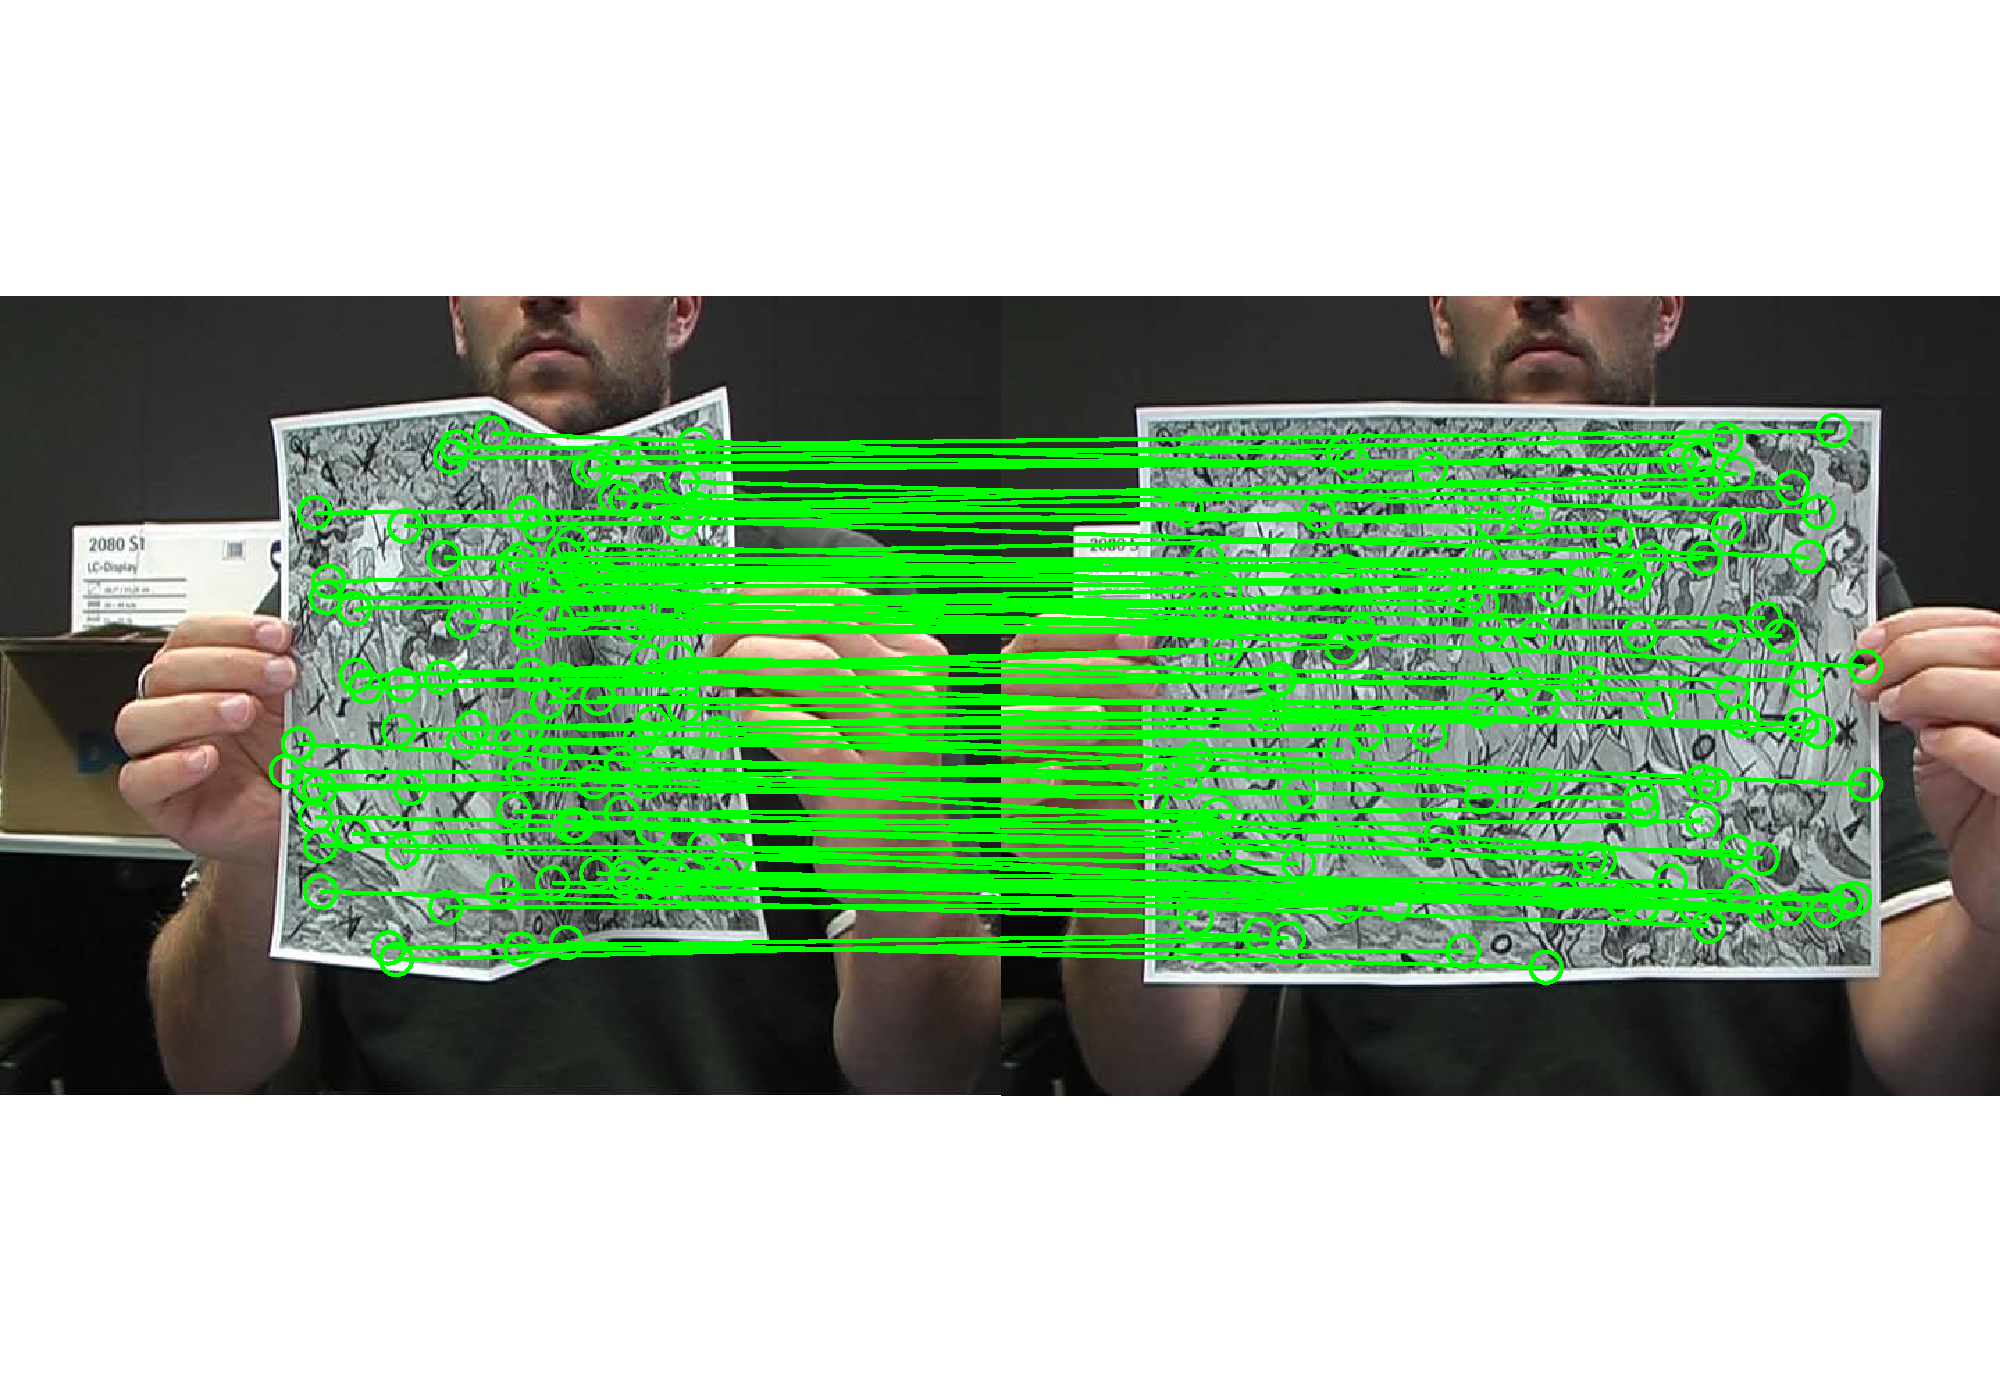
\includegraphics[width=0.6\linewidth]{figures/teaser3.pdf}
   \caption{Correspondences between 3D datasets determined by SuperMatching, using combined SIFT features (for color) and slippage features (for geometry).
   %%%RRM SIFT for colour, slippage for geometry? From 3D input?
   %%%RRM check I understood this right.
   Left: rigid pairwise matching of views of a colored jug. Right: matching of a unfolded piece of paper with a large deformation.}
}
%%% The ``\maketitle'' command must appear after ``\begin{document}'' and,
%%% if you have one, after the definition of your ``teaser'' image, and
%%% before the first ``\section'' command.

\maketitle

%%% Your paper's abstract goes in its own section.

\begin{abstract}
We present a feature matching algorithm for finding correspondences between two sets of features.
Our approach is based on finding matching triangles and quadrangles, going beyond the single (point) and pairwise (segment) of features typically used.
Our algorithm is formulated as supersymmetric-tensor-based higher-order matching scheme,
the higher-order affinity measures taking into account matches between more than a single or pairwise features.
We exploit a compact form of this affinity tensor, taking advantage of supersymmetry to devise an efficient sampling strategy to create the affinity tensor.
Matching is performed using the rank-one approximation of the tensor directly with a higher-order power method.
Experiments on both synthetic and real RGB images and depth videos show that
our algorithm provides accurate and robust matching of feature correspondences in the complex scenario.

\end{abstract}

%%% ACM Computing Review (CR) categories.
%%% See <http://www.acm.org/class/1998/> for details.
%%% The ``\CRcat'' command takes four arguments.

%\begin{CRcatlist}
%  \CRcat{I.3.7}{Computer Graphics}{Three-Dimensional Graphics and Realism}{Radiosity};
%\end{CRcatlist}

%%% The ``\keywordlist'' command prints out the keywords.

\keywordlist

%%% The ``\TOGlinkslist'' command will insert hyperlinked icon(s) to your
%%% paper. This includes, at a minimum, hyperlinked icons to the ACM article
%%% page and the ACM Digital Library-held PDF. If you added URLs to
%%% ``\TOGprojectURL'' or the other, similar commands, they will be added to
%%% the list of icons.
%%% Note: this functionality only works for annual-conference papers.

%\TOGlinkslist

%%% The ``\copyrightspace'' command
%%% Do not remove this command.

\copyrightspace

%%% This is the first section of the body of your paper.
\section{Introduction}
\label{sec:introduction}

Building correspondences between two sets of features of 2D/3D shapes is a fundamental problem in many geometric processing,
computer graphics and computer vision tasks.
It arises in applications such as feature extraction~\cite{Johnson99,Lowe04,Sun09,Bokeloh08,Toler10,Leutenegger11},
shape matching~\cite{Berg05,Brown07,Lorenzo08,Tevs09,Ovsjanikov10,Tevs11,SahilliogluY11,Windheuser11}, registration of 3D shapes~\cite{Gelfand05,Aiger08,li08,Zeng10,vanKaick11,Chang11},
automatic shape understanding~\cite{Lipman09,Sun10,Kim11}, shape retrieval from database~\cite{Bronstein11}, and reconstruction~\cite{Brown07,Chang11}.

In principle and practise, the correspondence building process mainly proceed in three steps~\cite{Lowe04,Leutenegger11}:
salient feature detection, high-quality descriptor, and accurately matching.
The former two problems have been been widely attracted considerable attention as their importance is easy perceivable.
However, even with the ideal feature detector and descriptor that capturing the most important and distinctive information content enclosed in the detected salient regions,
the correspondences still could not ideally built in the state-of-the-art algorithms~\cite{vanKaick11}.
The reason is that the real input data is so inperfect and complex especially with symmetric and repetitive regions.
The researchers are beginning to be aware of that the limitation could be effectively alleviated by feature matching.
Some original idea (e.g. RANSAC-like algorithms~\cite{Tevs09,Tevs11}) has been extended,
or indirectly sorting to shape embedding strategies, such as Generalized Multidimensional Scaling~\cite{Bronstein11},
Heat Kernel Map~\cite{Ovsjanikov10}, M{\"o}bius Transformation~\cite{Lipman09,Kim11}.
But, these previous algorithms still did not treat feature matching as one independent problem,
although they agreed with that matching is not tightly coupled with feature detection and description.

In the paper, we mainly focus on feature matching problem, which is complementary to existing feature detection and desription algorithms.
As we know, a matching itself may comprise one or more items of a given kind.
We may match single point to single point (point-single),
point pairs separated by a fixed distance to other point pairs (segment-double),
triples of points forming a triangle to other triples of points (triangle-triple),
quadruples of points forming a quadrangle to other quadruples of points (quadrangle-quadruple), and so on.
As pointed by~\cite{Conte04}, when single features are matched,
we must solve a linear assignment problem, if multiple features are matched at once,
a quadratic or higher-order assignment problem results.

Linear assignment matches single features in one set with single features in the other set, and could be mainly treated as single points linkage.
Matching two feature sets by considering similarities of \emph{single} features from each set can easily fail in the presence of ambiguities such as repeated elements,
or similar local appearance.

Quadratic and higher-order assignment matches groups of features in one set simultaneously with groups from the other set,
and requires a greater consistency between the information being matched, making it more reliable.
As well as the features themselves, other constraints such as consistency of the distances between the features being matched are also enforced,
greatly improving the matching accuracy.

As a particular example of \emph{quadratic} assignment, Leordanu and Hebert~\cite{Leordeanu05} consider pairs of feature descriptors,
and distances between pairs of features from each set to reduce the number of incorrect correspondences.
Such pairwise distance constraints are particularly helpful in cases when the features themselves have low discriminative ability.
The idea has been widely adopted in the 3D shape matching algorithms~\cite{Tevs09,Ovsjanikov10,Tevs11,Kim11,SahilliogluY11,Windheuser11}.

Higher-order assignment further generalizes the assignment problem to include yet more complex constraints between features.
For example, third-order potential functions, proposed in~\cite{Duchenne09,Zeng10,Chertok10},
quantify the affinity between two point triples by measuring the similarity of the angles formed by such two feature tuples (triangles).
However, this angular similarity value only calculates the total differences in corresponding angles,
and does not change with the order of the input assignments.
By changing the affinity tensor to a \emph{supersymmetric} tensor~\cite{Kofidis02}, the unaccurate limitation could be further solved by our algorithm.

Thus, by formulating the higher-order problem using a supersymmetric affinity tensor,
we propose a general higher-order supersymmetric matching algorithm, named \emph{SuperMatching}.
SuperMatching, addressed in Section~\ref{sec:supersymhopm}, which accurately matching a moderate number of features using triples or higher polygons of features.
The contributions of this paper include:
\begin{itemize}
\item We show how to define a compact higher-order supersymmetric affinity tensor to express geometric consistency constraints between tuples of features.

\item Based on the supersymmetry of the affinity tensor, we propose a higher-order power iteration method, which efficiently solves the matching problem.

\item The affinity tensor is physically created by using a new efficient sampling strategy for feature tuples,
which avoids sampling repetitive items, reduces the number of feature tuples to be sampled while improving the matching accuracy.

\end{itemize}

Our experiments in Section~\ref{sec:experiments} on both synthetic and real captured data sets show that SuperMatching result is accurate and robust,
and has competitive computational cost compared to previous algorithms.
More important, the matching is performed by incorporating variant 2D and 3D feature descriptors,
which demonstrate that SuperMatching is independent on descriptors and could be generally applied in computer graphics and computer vision fields.

%Section~\ref{sec:supersymhopm} describes the higher-order supersymmetirc affinity tensor and the power iteration method.
%Experiments are shown in Section~\ref{sec:experiments} and conclusions drawn in Section~\ref{sec:conclusion}. 
\section{Related work}
\label{sec:related}

Finding correspondences between two sets of discrete features, such as points, is a classical problem, and thus there is a large literature on the subject.
Previous approaches can be classified into the which match single points to single points, those which match pairs of points to pairs of points, and so on.

Matching single points to single points, i.e.\ linear assignment problems, only consider affinity measures between two graph nodes, one from each set being matched, typically the feature distance between the two feature points.
In concrete terms, the linear assignment problem is posed as: find a mapping $f:\ P_1\to P_2$,
such that the optimal assignment $S^*=\argmax\sum\nolimits_{i\in P_1}A(i,j(i))$,
where $A:\ N_1\times N_2 \to R$ is the \emph{affinity matrix}, and $A(i,j)$ measures the affinity between feature $i\in P_1$ and feature $j\in P_2$.
%%%RRM Need to say the mapping is one to one?
Such affinity measures rely heavily on descriptors computed using local information around each feature point
(e.g.\ shape contexts~\cite{Belongie02}, SIFT~\cite{Lowe04}, spin images~\cite{Johnson99}, heat diffusion signatures~\cite{Sun09}) in many computer vision and geometric computing tasks.
It is apparent that point-to-point matching is weak in that wrong correspondences maybe readily be established.

Matching pairs of points in one set to pairs of points in the other set leads to a quadratic assignment problem.
We now have an affinity matrix $A: N_1N_2\times N_1N_2 \to R$, where $A(i,j)$ measures the compatibilities between two assignments $s_i=(f_i^1,f_{j(i)}^2)$ and $s_j=(f_i'^1,f_{j^{'}(i')}^2)$,
which takes into account both similarity of point features \emph{and} Euclidean distance between the points in a pair.
The quadratic assignment problem seeks to find a mapping $f:\ P_1\to P_2$ which represents the optimal assignment.
Unfortunately, this problem is NP-hard, but spectral relaxation techniques~\cite{Leordeanu05} can provide good approximate solutions.

Several higher-order constraints beyond pairwise potentials
%%%RRM why do you call them potentials? Not explained or defined yet.
have been proposed.
In general, we may define an $m^{th}$-order affinity measure $T_m$ to capture the affinity associated with making $m$ particular simultaneous assignments $s_{i_1}=(f_{i_1}^1,f_{j_1(i_1)}^2,),\; \cdots \;,s_{i_m}=(f_{i_m}^1,f_{j_m(i_m)}^2)$.
Such higher-order methods can significantly improve matching accuracy, 
but the higher-order assignment problem is again NP-hard, and various approximate methods have again been developed.
Zass and Sashua~\cite{Zass08} consider a probabilistic model of soft hypergraph matching.
They reduce the higher-order problem to a first-order one by marginalizing the higher-order tensor to a one dimensional probability vector.
Duchenne et al.~\cite{Duchenne_etal09} introduced a third-order tensor in place of an affinity matrix to represent affinities of feature triples,
and higher-order power iteration was used to achieve the final matching.
%%%RRM Need to say more here about how our method differs from this.
Chertok et al.~\cite{Chertok10} treat the tensor as a joint probability of assignments, marginalize the affinity tensor to a matrix,
and find optimal soft assignments by eigendecomposition of the matrix.
Wang et al.~\cite{Aiping10} also built a third-order affinity tensor and obtained a final matching by rank-one approximation of the tensor.
%%%RRM There are several methods above which we have used parts of. You need to
%%%RRM quite clearly say, for each paper seaparately
%%%RRM - which parts / ideas of these papers we have re-used
%%%RRM - how we have gone beyond them
Higher-order assignment problems typically require large amounts of memory and computational resources.
By reducing the number of elements needed to represent the affinity measures,
%%%RRM How is this reduction done?
the above approaches can efficiently match large numbers (many hundreds or more) of features.
However, these approaches sparsify the affinity information to some degree, leading to a reduction in matching accuracy.
When matching two feature sets with large differences in scale, the matching results may become unstable.
%%%RRM Why should the sets have large differences in scale? Surely most matching problems
%%%RRM are done with scale = 1?
%%%RRM Finish this by saying what our idea is that goes beyond these previous papers

A similar idea for 3D registration, called the 4-Points Congruent Sets method (4PCS), was proposed by Aiger et al.~\cite{Aiger08}. 
It is a fast and robust alignment scheme for 3D point sets that uses widely separated point tuples, providing resilience to noise and outliers.
The key geometric idea is that 4PCS defines a ratio property which is preserved for planar 4-point sets under affine transformations.
We use similar geometric rules in a more general way for feature matching.
%%%RRM be more specific about how we are more general.


%%==========================================================================
\section{Overview}
\label{sec:overview}

A tensor generalizes vectors and matrices to higher dimensions: a vector is a tensor of order one,
and a matrix is a tensor of order two. A higher-order tensor can be expressed as a multi-dimensional array~\cite{Kolda08}.
More formally, an $N$th-order tensor is an element of the tensor product of $N$ vector spaces, each of which has its own coordinate system.

Assume we are given two sets of feature points $P$ and $Q$, with $N_1$ and $N_2$ points respectively.
From the $N$th-order tensor viewpoint, the matching between these two feature sets can be represented by an \emph{assignment variable} $\boldsymbol{x}$.
The matching problem is equivalent to finding the optimal assignment tensor ${\boldsymbol{x}}^*=<x_{i_1},\cdots,x_{i_N}>
 \in \{0,1\}^{N}$, satisfying~\cite{Kolda08,Duchenne09}
\begin{equation}
\label{equ:assigment}
  {\boldsymbol{x}}^* = \argmax_{\boldsymbol{x}}  \sum_{i_1,\cdots,i_N} \mathcal{T}_N(i_1,\cdots,i_N) x_{i_1}  \cdots\; x_{i_N}.
\end{equation}

Here, $i_n \in \{i_1,\cdots ,i_N\}$ stands for an assignment in $n$th index/dimension of the $N$ vector spaces.
Let all feature tuples for $P$ and $Q$ be $F_1$ and $F_2$, then $\forall (f_{i_1}^1, \cdots, f_{i_N}^1)\in F_1$,
there exits a matching for $(f_{i_1}^1, \cdots, f_{i_N}^1)$ to its corresponding feature tuples in $F_2$.
For example, a third-order tensor, $i_n \in \{1,2,3\}$, 
each index could be expressed as $i_1=(f_{i_1}^1,f_{i_1}^2), i_2=(f_{i_2}^1,f_{i_2}^2), i_3=(f_{i_3}^1,f_{i_3}^2)$ pairs of potentially matched points.
The product $x_{i_1} \cdots\;x_{i_N}$ will be equal to $1$ if the points $(f_{i_1}^1, \cdots, f_{i_N}^1)$ are all matched to the points $(f_{i_1}^2, \cdots, f_{i_N}^2)$, 
and otherwise 0.
$\mathcal{T}_N(i_1,\cdots,i_N)$ is the affinity of the set of assignments $\{i_n\}_{n=1}^N$, 
which will be high if the sets of features $(f_{i_1}^1, \cdots, f_{i_N}^1)$  are similar to the set $(f_{i_1}^2, \cdots, f_{i_N}^2)$.
Note that the size of $\mathcal{T}_N(i_1,\cdots,i_N)$ is ${(N_1N_2)}^N$.
In the paper, \emph{the affinity measures would be defined based on the supersymmetric tensor to express the geometric constraints between pairs of feature tuples},
this is the basis of our SuperMatching algorithm.

In the rest of the paper, we consider the one-to-many correspondence problem.
We assume that each point in $P$ is matched to exactly one point in $Q$, but that the reverse is not necessarily true.
If \emph{do} we want to treat both datasets in the same way,
we can first match $P$ to $Q$, then match $Q$ to $P$, and then combine the matching results by taking their union or intersection.

From Equ.(\ref{equ:assigment}) we can see that there are four issues to be considered when using higher-order matching algorithms. How should we:
\begin{itemize}
\item organize and express the affinity measures $\mathcal{T}_N$ in a supersymmetric manner? (see Section~\ref{subsec:supersymtensor})
\item approximately solve the optimal higher-order assignment problem efficiently? (see Section~\ref{subsec:oursymmhopm})
\item define the affinity measure between two feature tuples? (see Section~\ref{subsec:potentials})
\item determine an appropriate sampling strategy to estimate the affinity tensor in a way which will give good matching accuracy? (see Section~\ref{subsec:sampling})
\end{itemize}




%%==========================================================================
\section{SuperMatching}
\label{sec:supersymhopm}
%-------------------------------------------------------------------------
We now discuss the first two issues mentioned above, which are independent of application; later we turn to definition of affinity measure, which is application dependent, and sampling strategy.


\subsection{Supersymmetric Affinity Tensor}
\label{subsec:supersymtensor}

Here we consider the supersymmetric higher-order affinity tensor, which is invariant under permutation of indices.
The main motivation of using supersymmetry is to allow us to avoid redundant storage and computation.

\newtheorem{mot}{Definition}
\begin{mot}[Supersymmetric Tensor]
\label{mot:def1}
A tensor is  \emph{supersymmetric} if its entries are invariant under any permutation of its indices~\cite{Kofidis02}.
\end{mot}

For example, a third-order supersymmetric tensor $\mathcal{T}_3$, satisfies the relationships:
$\mathcal{T}_3(i_1, i_2, i_3)=\mathcal{T}_3(i_1, i_3, i_2)=\mathcal{T}_3(i_2, i_1, i_3)=\mathcal{T}_3(i_2, i_3, i_1)=\mathcal{T}_3(i_3, i_1, i_2)=\mathcal{T}_3(i_3, i_2, i_1)$.

\begin{mot}[Supersymmetric Affinity Tensor]
\label{mot:def2}
Given two feature sets $P$ and $Q$, with $N_1$ and $N_2$ features respectively,
the supersymmetric affinity tensor is an $N$th order $I_1, \cdots, I_N$, nonnegative tensor $\mathcal{T}_N$,
for which there exists a set of indices $\theta_N$,
and an $N$th order potential function $\phi_N$, such that
%
\begin{flalign}
\mathcal{T}_N(i_1,\ldots,i_N) = \begin{cases}
\phi_N(\Omega(i_1,\ldots,i_N))&{,\forall(i_1,\ldots,i_N)\in \theta_N}  \\
\quad{}\quad{}\quad{}   0     &{,\forall(i_1,\ldots,i_N)\notin \theta_N}
\end{cases}
\end{flalign}
%
where $\Omega$ stands for an arbitrary permutation of the vector, and $\theta_N$ satisfies $\forall (i_1,\ldots,i_N)\in \theta_N, \forall i_m\in\{i_1, \ldots, i_N\}$
and $\forall i_n\in\{i_1, \ldots, i_N\}-\{i_m\}$ meets the requirement that $i_m \neq i_n$.
\end{mot}

A tensor element with $(i_1,\ldots,i_N)\in \theta_N$ is called a \emph{potential element}, while other elements are called \emph{non-potential element}.
A potential element is one real matching result out of all possible matching candidates.
\cz{The potential elements would be further detailed in the Section~\ref{subsec:sampling}.}

%%%RRM It is still not clear why there are non-potential elements - this means you do not permit some possible matching results. Why?
%%%ZQC If one element whose components are not invariant, then it would not be one potential element.
%%%YKL I think potential/non-potential elements are related to sampling? You can refer to Section 4.4 to make it clearer.

Using Definition~\ref{mot:def2}, we now can reduce the amount of storage needed, representing every potential element $\mathcal{T}_N(i_1,\ldots,i_N)$ by the canonical entry $\mathcal{T}_N(\mathrm{sort}(i_1,\ldots,i_N))$, $\forall (i_1,\ldots,i_N)\in \theta_N$. Each stored value thus provides the value for $N!$ entries.
Furthermore, as non-potential elements all have value zero, there is no need to store them.
This greatly reduces both storage, and the amount of feature tuple sampling
needed  when estimating the affinity tensor, as discussed in Section~\ref{subsec:sampling}.
At the same time, it can be used to make the power iteration process more efficient: see Section~\ref{subsec:oursymmhopm}.

%-------------------------------------------------------------------------
\subsection{Supersymmetric Higher-order Power Iteration}
\label{subsec:oursymmhopm}

\begin{algorithm}[!t]
\caption{\small Higher-order power iteration solution for the \protect\\
         \mbox{}\hspace{15ex}\small supersymmetric affinity tensor (with $\mathcal{C}_1$ norm)}
\label{alg2}
\begin{algorithmic}[1]
\REQUIRE \small $N^{th}$-order supersymmetric affinity tensor
\ENSURE  \small Unit $\mathcal{\ell}^1$-norm vector $\boldsymbol{u}$
\STATE   \small \; Initialize $\boldsymbol{u}_0$ by randomly positive values, $k=1$
\REPEAT
    \FOR{all $(i_1,i_2,\cdots , i_N)\in \theta_N$}
        \FOR{all $m \in (i_1,\cdots , i_N)$}
        \STATE $v_{m}^{(k)}=(N-1)!\phi_N(i_1,\cdots , i_N) 2v_{m}^{(k-1)}v_{i_1}^{2_{(k-1)}}\cdots$ \\
                 $\qquad \qquad v_{m-1}^{2_{(k-1)}}v_{m+1}^{2_{(k-1)}}\cdots v_{i_N}^{2_{(k-1)}}$
        \ENDFOR
        \FOR{$i=1:N_1$}
        \STATE $v^{(k)}(((i-1)\cdot N_2+1) : i\cdot N_2)=$   \protect\\
               $\hat{v}^{(k)}(((i-1)\cdot N_2+1) : i\cdot N_2)/\lVert \hat{v}^{(k)}(((i-1)\cdot N_2+1):i\cdot N_2)\lVert_1$
        \ENDFOR
    \ENDFOR
    \STATE $k=k+1$;
\UNTIL{\small convergence};\protect\\
       \small \textbf{Note}: $\boldsymbol{u}^{(k)}=\boldsymbol{v}^{2_{(k)}}$, $\phi_N$ is the corresponding potential function,
       \small and $v^{(k)}(((i-1)\cdot N_2+1) : i\cdot N_2)$ denotes the slice of $v^{(k)}$ with
       \small indices from $(i-1)\cdot N_2+1$ to $i\cdot N_2$.
\end{algorithmic}
\end{algorithm}

The higher-order tensor problem in Eq. (\ref{equ:assigment}) may be solved by the tensor decomposition method~\cite{Kolda08}.
Tensor decomposition originated in~\cite{Hitchcock27}.
We utilize the rank-one higher-order power method~\cite{Lathauwer95} to approximately solve the Equ.(\ref{equ:assigment}); as noted, an exact computation is infeasible.
So, Equ.(\ref{equ:assigment}) can be expressed as:
\begin{eqnarray}
\label{equ:assigment2}
{\boldsymbol{x}}^* &=& \argmax_{\boldsymbol{x}} \sum_{i_1,i_2,\cdots,i_N} \mathcal{T}_N(i_1,\cdots,i_N) x_{i_1} \cdots x_{i_N} \nonumber\\
&=& \max <\mathcal{T}_N, \boldsymbol{x}^{\star N}>
\end{eqnarray}
where $\star$ is called the Tucker product~\cite{Kofidis02}, and $\boldsymbol{x} \in \{0,1\}^{N}$.
To get an approximate solution, we relax the constraints:
the binary assignment vector $\boldsymbol{x}\in \{0,1\}^{N}$ is replaced by an assignment vector $\boldsymbol{u}$ with elements taking real values in $[0,1]$.
This changes the optimization problem to one of computing the rank-one approximation of the affinity tensor $\mathcal{T}_N$~\cite{Kofidis02},
i.e.\ finding a scalar $\lambda$ and a unit norm vector $\boldsymbol{u}\in \mathbb{R}^{N}$,
such that the tensor $\hat{\mathcal{T}_N} = \lambda \boldsymbol{u}\star \boldsymbol{u} \star\cdots \star \boldsymbol{u}=\boldsymbol{u}^{\star N}$ minimizes the Frobenius norm squared function $f(\hat{\mathcal{T}_N})=\lVert \mathcal{T}_r-\hat{\mathcal{T}_N} \lVert^2_F$.
The final matching result is found by replacing each element of $\boldsymbol{u}$ by 0 or 1 according to whichever it is closer to.

The higher-order power method is commonly used to find the rank-one tensor approximation;
a version for supersymmetric tensors (S-HOPM) is given in~\cite{Kofidis02}.
The S-HOPM algorithm converges under the assumption of convexity (or concavity) for the functional induced by the tensor~\cite{Kofidis02},
which is sufficiently robust for practical applications.
S-HOPM is performed in two iterative steps: higher-order power iteration of $\boldsymbol{u}$, followed by normalization of $\boldsymbol{u}$ under the Frobenius norm.
A recent effective improvement~\cite{Duchenne09} uses the $\mathcal{\ell}^1$ norm to replace the traditional $\mathcal{\ell}^2$ norm.

We both use the $\mathcal{\ell}^1$ norm, and further revise S-HOPM as follows.
To perform higher-order power iteration of $\boldsymbol{u}$, we must compute $\hat{\boldsymbol{u}}^{(k)}=\mathcal{I}\mathop{\star}\limits^{\mathcal{T}_N}
{(\boldsymbol{u}^{(k-1)})}^{\mathop{\star}\limits^{\mathcal{T}_N} (N-1)}$, where
$\mathop{\star}\limits^{\mathcal{T}_N}$ is a so-called $\mathcal{T}_N$-product,
and $\mathcal{I}$ is the unit tensor~\cite{Kofidis02}.
For $\hat{\boldsymbol{u}}^{(k)}$ belonging to an $N{th}$-order supersymmetric affinity tensor, this can be formulated as follows:
%\begin{small}
\begin{flalign}
\label{equ:eqsmain2}
&\hat{\boldsymbol{u}}^{(k)}=\mathcal{I}\mathop{\star}\limits^{\mathcal{T}_N}
{(\boldsymbol{u}^{(k-1)})}^{\mathop{\star}\limits^{\mathcal{T}_N} (N-1)} \mathrm{~implies~that~} \forall m\in (i_1,... , i_N), \nonumber \\
&v_{m}^{(k)}= \nonumber\\
&\sum\limits_{i_1,...,i_N}\mathcal{T}_N(i_1,...,i_N)2v_{m}^{(k-1)}v_{i_1}^{2_{(k-1)}}... v_{m-1}^{2_{(k-1)}}v_{m+1}^{2_{(k-1)}}... v_{i_N}^{2_{(k-1)}}= \nonumber \\
&(N-1)!\phi_N(i_1,...,i_N)2v_{m}^{(k-1)}v_{i_1}^{2_{(k-1)}}... v_{m-1}^{2_{(k-1)}}v_{m+1}^{2_{(k-1)}}... v_{i_N}^{2_{(k-1)}}
\end{flalign}
%\end{small}
where $\boldsymbol{u}^{(k)}=\boldsymbol{v}^{2_{(k)}}$, and $\phi_N$ is the corresponding potential function that would be detailed in the following Section~\ref{subsec:potentials}.

Note that Eq. (\ref{equ:eqsmain2}) is more compact than earlier expressions in the literature, as it handles all symmetrically related potential elements as a single item using   multiplication by $(N-1)!$.
%%%RRM But if N is 3, (N-1)! is just 2, so this only gives a speed improvement of 2?
%%%ZQC You are right Ralph, only 2 :) for each element, however there are many elements.
The efficiency of our SuperMatching algorithm relies on two principles.
First, we take advantage of the supersymmetry to deduce $\boldsymbol{u}$ as in Equ.(\ref{equ:eqsmain2}).
Secondly, many of the elements of the affinity tensor are zero non-potential elements, and it is much more efficient to perform the power iteration by just considering the non-zero potential elements.

Our supersymmetric higher-order power iteration solution of Eq. (\ref{equ:assigment}) is performed by the SuperMatching algorithm---See Algorithm~\ref{alg2}.
It excludes each non-potential element from the iteration process and only utilizes one canonical potential element for each related element, so it is efficient.
The complexity of the whole iteration process only depends on the number $|\theta_N|$ of non-zero affinities. Step 5 in Algorithm~\ref{alg2} represents all permutations of each potential element $\mathcal{T}_N(i_1,\cdots,i_N)$
using a single potential function $\phi_N(i_1,\cdots,i_N)$.
Consequently, this method reduces memory costs while keeping accuracy.
Note that, although~\cite{Duchenne09} claimed to use a supersymmetric affinity tensor,
his approach does not make full use of supersymmetry when creating the supersymmetric affinity tensor,
nor does it take advantage of supersymmetry to accelerate the power iteration process.
By doing so, we overcome limitations due to unbalanced and redundant tensor elements in~\cite{Duchenne09}, as our experiments show later.

Many initialization schemes have been proposed for the S-HOPM method~\cite{Kofidis02}.
We simply use positive random values between $0$ and $1$ to initialize $\boldsymbol{u}_0$, which ensures convergence; proofs are detailed in~\cite{Regalia00,Kofidis02}.

\subsection{Higher-order Potentials}
\label{subsec:potentials}

Different higher-order potentials are appropriate for different applications.
Here we give two general higher-order potentials.
One may be used for  2D cases, while the other is useful for 3D matching.
The potentials are based on a Gaussian function
which guarantees the tensor elements are non-negative and invariant under any permutation of the input assignments.

In 2D, we first restate a well-known 2D third-order geometric-similarity invariant potential $\phi_3$~\cite{Duchenne09,Chertok10} for linking two point feature triples.
Similarity of triangles formed by three points corresponds to invariance under scaling, rotation and translation---interior angles do not change.
Thus $\phi_3$ can be defined in terms of differences of corresponding interior angles:
\begin{eqnarray}
\phi_3(i_1,i_2,i_3)&=&\phi_3(\{p_1,q_1\}, \{p_2,q_2\}, \{p_3,q_3\})\nonumber\\
&=&\exp(-1/\varepsilon^2\sum\nolimits_{(l,l^{'})}\lVert \alpha_l- \alpha_{l^{'} } \lVert^2 )
\end{eqnarray}
where $\varepsilon > 0$ is the is the kernel bandwidth,
$\{\alpha_l\}_{l=1}^3$ and $\{\alpha_l^{'}\}_{l^{'}=1^{'}}^{3}$ are the angles formed by feature triples $(p_1,p_2,p_3)$ and $(q_1,q_2,q_3)$:
see Figure~\ref{fig:TO}. Each point corresponds to one interior angle.
We may extend it to the general case by using the internal angles formed by  polygons with more than 3 sides.
It is easy to see that the potential preserves invariance under rigid transformations in 2D field.

For 3D matching problems, we may replace the internal angle by edge length, i.e.\ the geodesic distance across the mesh in which the points are embedded. which now corresponds to assuming
an isometry transform relating the point sets.
Geodesic distance may be computed by  Dijkstra's algorithm~\cite{Peyre2010} .

We will use these two high-order potentials to evaluate our algorithm.
Figure~\ref{fig:TO} illustrates the  third-order potential examples in the 2D and 3D cases.

\begin{figure}
\centering
  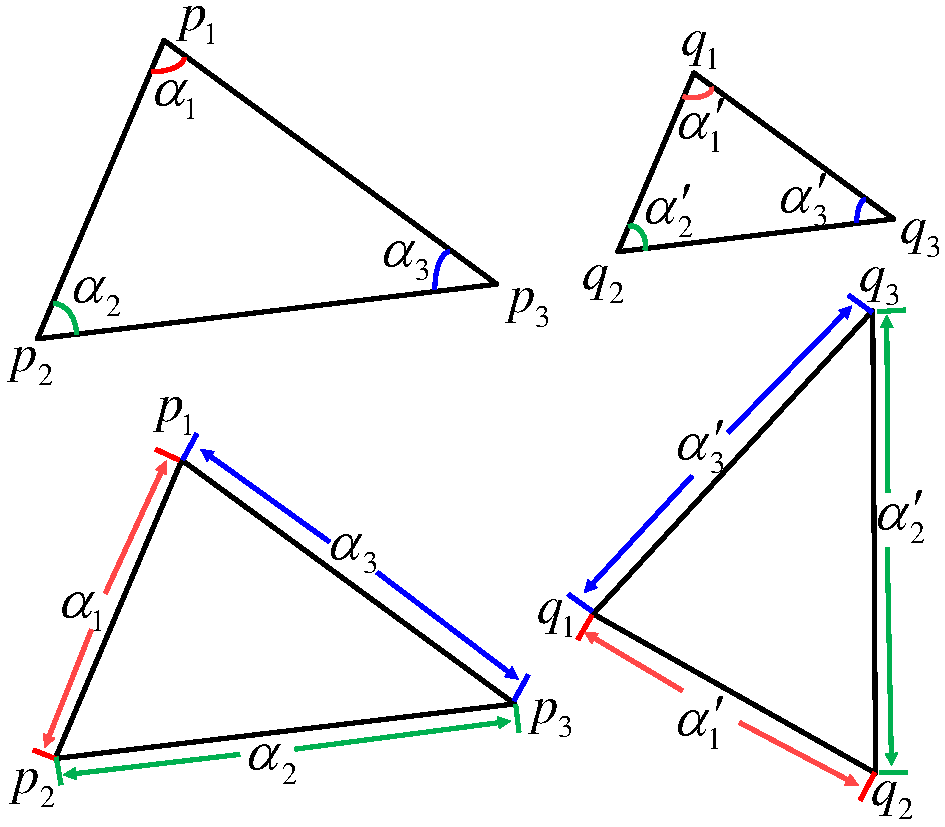
\includegraphics[width=0.7\linewidth]{figures/diagram.pdf}
  \caption{Third-order potential. The geometric constraints are: internal angle invariance in 2D (above), and edge length invariance in 3D (below).}
\label{fig:TO}
\end{figure}

%-------------------------------------------------------------------------
\subsection{Sampling Strategy}
\label{subsec:sampling}

Algorithm~\ref{alg2} depends on all potential elements.
We next discuss the issue of how to sample the feature tuples to build potential items, which determines the size $|\theta_N|$ and influences matching accuracy.

For the two feature sets $P$ and $Q$,
a potential element may be obtained by using two feature tuples sampled from each feature set separately.
For $N^{th}$-order matching, a naive way to construct the potential elements is as follows:
first find all feature tuples for $P$ and $Q$, as $F_1$ and $F_2$; then $\forall (f_{i_1}^1, \cdots, f_{i_N}^1)\in F_1$,
calculate the potentials for $(f_{i_1}^1, \cdots, f_{i_N}^1)$ with all feature tuples in $F_2$.
This naive method is very time-consuming, which is why sampling is used.
We employ random sampling for general feature matching problems,
but this does not preclude more directed sampling if prior knowledge of the matching problems gives guidance.

Our sampling approach is to repeatedly randomly sample $t_1$ feature tuples for each feature point from $P$, and fully sample $Q$.
For $P$, we repeatedly take one feature as a required element, and then randomly choose $t_1$ feature tuples containing this required element.
We repeat this process until all features in $P$ have been chosen once as a required element.
So the number of feature tuples in $F_1$ is $N_1t_1$, and $N_2^N$ for $F_2$.
Then, $\forall (f_{i_1}^1, \cdots, f_{i_N}^1)\in F_1$, we find $k$ most similar features in $F_2$ to build $N$ potential elements as $\phi_i^k$.
Combining all the potential elements obtained, we form the desired potential element set $\theta_N = \{\phi_i^k\}_{i=1}^{N_1 t_1}$, of size $|\theta_N| = N_1 t_1 k$.
\cz{For $P$, the sampling cost is $O(N_1 \, t_1 \, k \, logN_2)$.}
%%%YKL To find the k-nearest featurs from F2 may take an additional O(N2) complexity?
%%%ZQC you are right, it should be log(N_2).
The parameters $t_1$ and $k$ must be chosen according to the size of the feature sets.
In practice, for two feature sets each with hundreds points,
we may take $t_1 \approx 100$ and $k\approx300$ for third-order matching.
Our experiments demonstrate that this sampling approach works well.

An important aspect of our sampling approach is to use the supersymmetry of the affinity tensor. Potential elements whose indices are permutations of each other
have the same value, so should not be repeatedly sampled.
Thus, we use a sampling constraint that the sets of feature tuples $F_1$ obtained from the sampling process should have no repetition, in the sense that
\begin{eqnarray}
\label{equ:noredun2}
\forall (f_{i_1}^1,f_{i_2}^1,\cdots,f_{i_N}^1),(f_{j_1}^1,f_{j_2}^1,\cdots,f_{j_N}^1) \in F_1,\nonumber\\ (f_{i_1}^1,f_{i_2}^1,\cdots,f_{i_N}^1)\neq\Omega(f_{j_1}^1,f_{j_2}^1,\cdots,f_{j_N}^1)
\end{eqnarray}
where $\Omega$ is an arbitrary permutation.

%%%YKL How about [Wang et al. 2010]?
%%%ZQC Wang has the similar limitation.
\cz{Earlier work~\cite{Zass08,Duchenne09,Aiping10} adopted random sampling,}
but failed to impose any constraint on the sampling process to take into account supersymmetry,
leading to the possibility that feature tuples may be sampled multiple times.
For example, for third-order matching, it is possible that a feature tuple $(f_{i_1}^1, f_{i_2}^1, f_{i_3}^1)$ may be sampled from $P$ and $(f_{i_1}^2, f_{i_2}^2, f_{i_3}^2)$ from $Q$,
and also a feature tuple $(f_{i_1}^1, f_{i_3}^1, f_{i_2}^1)$ sampled from $P$ and $(f_{i_1}^2, f_{i_3}^2, f_{i_2}^2)$ from $Q$. That will create two tensor elements $\phi_3(s_{i_1}, s_{i_2}, s_{i_3})$ with index $(s_{i_1}, s_{i_2}, s_{i_3})$ and $\phi_3(s_{i_1}, s_{i_3}, s_{i_2})$ with index $(s_{i_1}, s_{i_3}, s_{i_2})$, which are the same. However, we just need one tensor element to express the affinity measure on the assignment group $(s_{i_1}, s_{i_2}, s_{i_3})$ for any permutation of indices.
This extra sampling is not only inefficient, but may also reduce the accuracy of the power iteration: one set of symmetrically related elements  may be represented by a different number of samples than another set of  symmetrically related elements, which unbalances the power iteration process, and can lead to inaccurate results.
Therefore, our sampling method reduces the sampling cost, while also improving the accuracy of the power iteration.

%%==========================================================================
\section{Experiments}
\label{sec:experiments}

We have used synthetically generated data as well as real captured data to evaluate the SuperMatching algorithm.
To demonstrate that the SuperMatching algorithm is general (independent of feature descriptors), several descriptors have been used.
For input shapes without color information, a uniform sampling of points on the source shape were employed.
For colored shapes, both SIFT feature points and uniform sampling points were used.
We used third-order matching in our experiments, and note it would be simple to use higher order.

%-------------------------------------------------------------------------
\subsection{3D Rigid Shapes Scans}
\label{subsec:3DRigid}

Firstly, we used SuperMatching to align 3D rigid shape scans pairwise based on the uniform sampling scheme.
Rigid transforms can be computed from three compatible sampling points.
The transform which brings the most data points within a threshold of a point in the model is chosen as the optimal aligning transform~\cite{Huttenlocher90}.
As discussed in~\cite{Gelfand05}, such a voting scheme is guaranteed to find the optimal alignment between the pairwise scans and is independent of the initial pose of the input scans.
Figure~\ref{fig:3DPair} shows some registration results for the Rooster model from~\cite{Chuang09}. On the left column is the original state,
then the following columns are our matching and registered result (without any ICP refinement~\cite{Besl92}); on the right column is the result produced by~\cite{Aiger08}.

\begin{figure}[htb]
\centering
  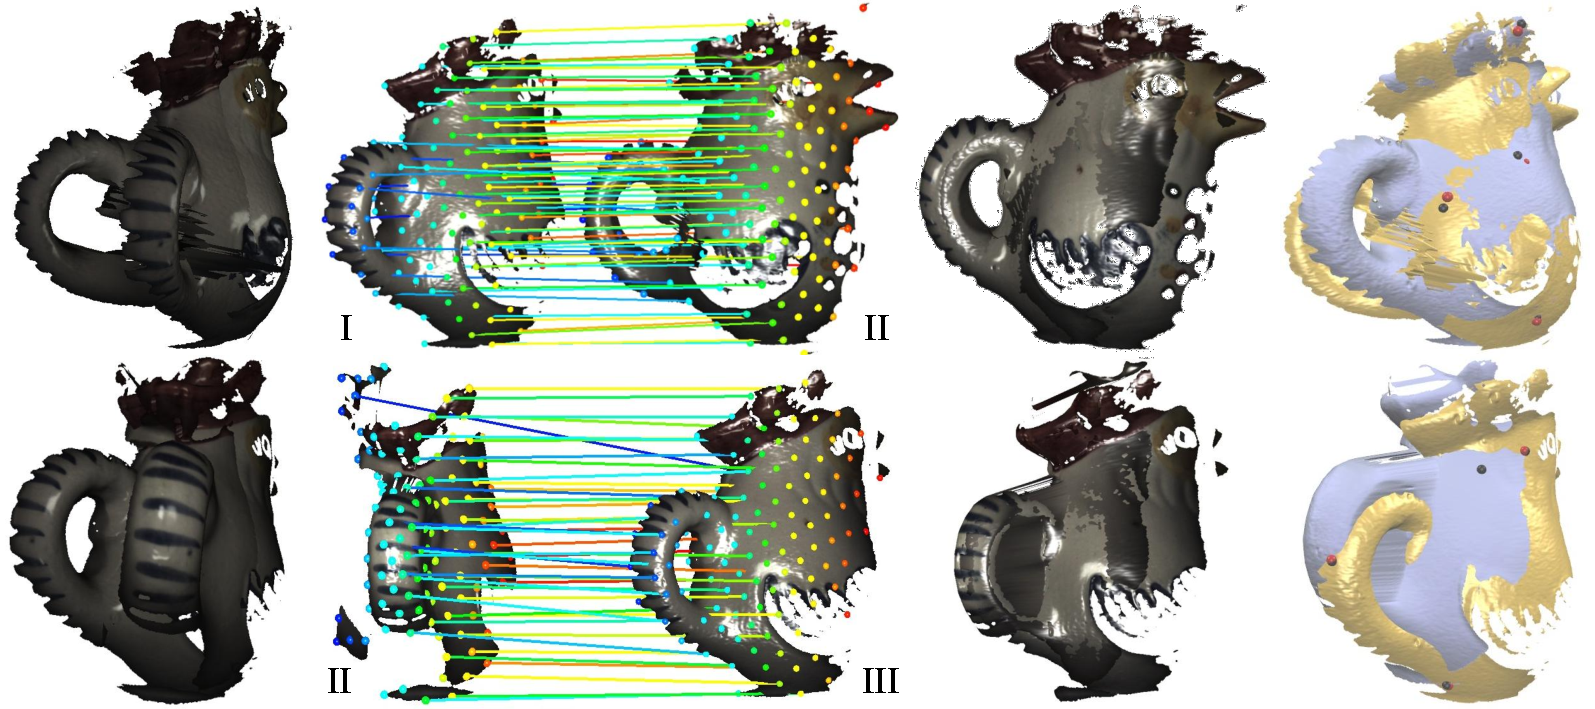
\includegraphics[width=0.99\linewidth]{figures/RoosterPair.pdf}
  \caption{Pairwise alignment of Rooster \emph{$I-II$} and \emph{$II-III$} scans. Left : our results. Right: results from [Aiger et al. 2008].}
\label{fig:3DPair}
\end{figure}

Next, we extended the SuperMatching to build a complete model from a set of scans from different viewpoints.
For these multiple scans,  third-order matching was first performed between each pair of consecutive scans.
After the initial pairwise matching, the alignment was refined by the iterative closest point (ICP) algorithm~\cite{Besl92}.
Figure~\ref{fig:3DRigid} illustrates the approach.
Above, a Rooster is aligned by our method, and the top-right is the real ground truth~\cite{Chuang09}.
Below, matching is used to align 8 partial scans which are then merged to produce a single shape.
Pairs of consecutive scans, linked by dark lines, are matched using the SuperMatching algorithm.

\begin{figure}[htb]
\centering
  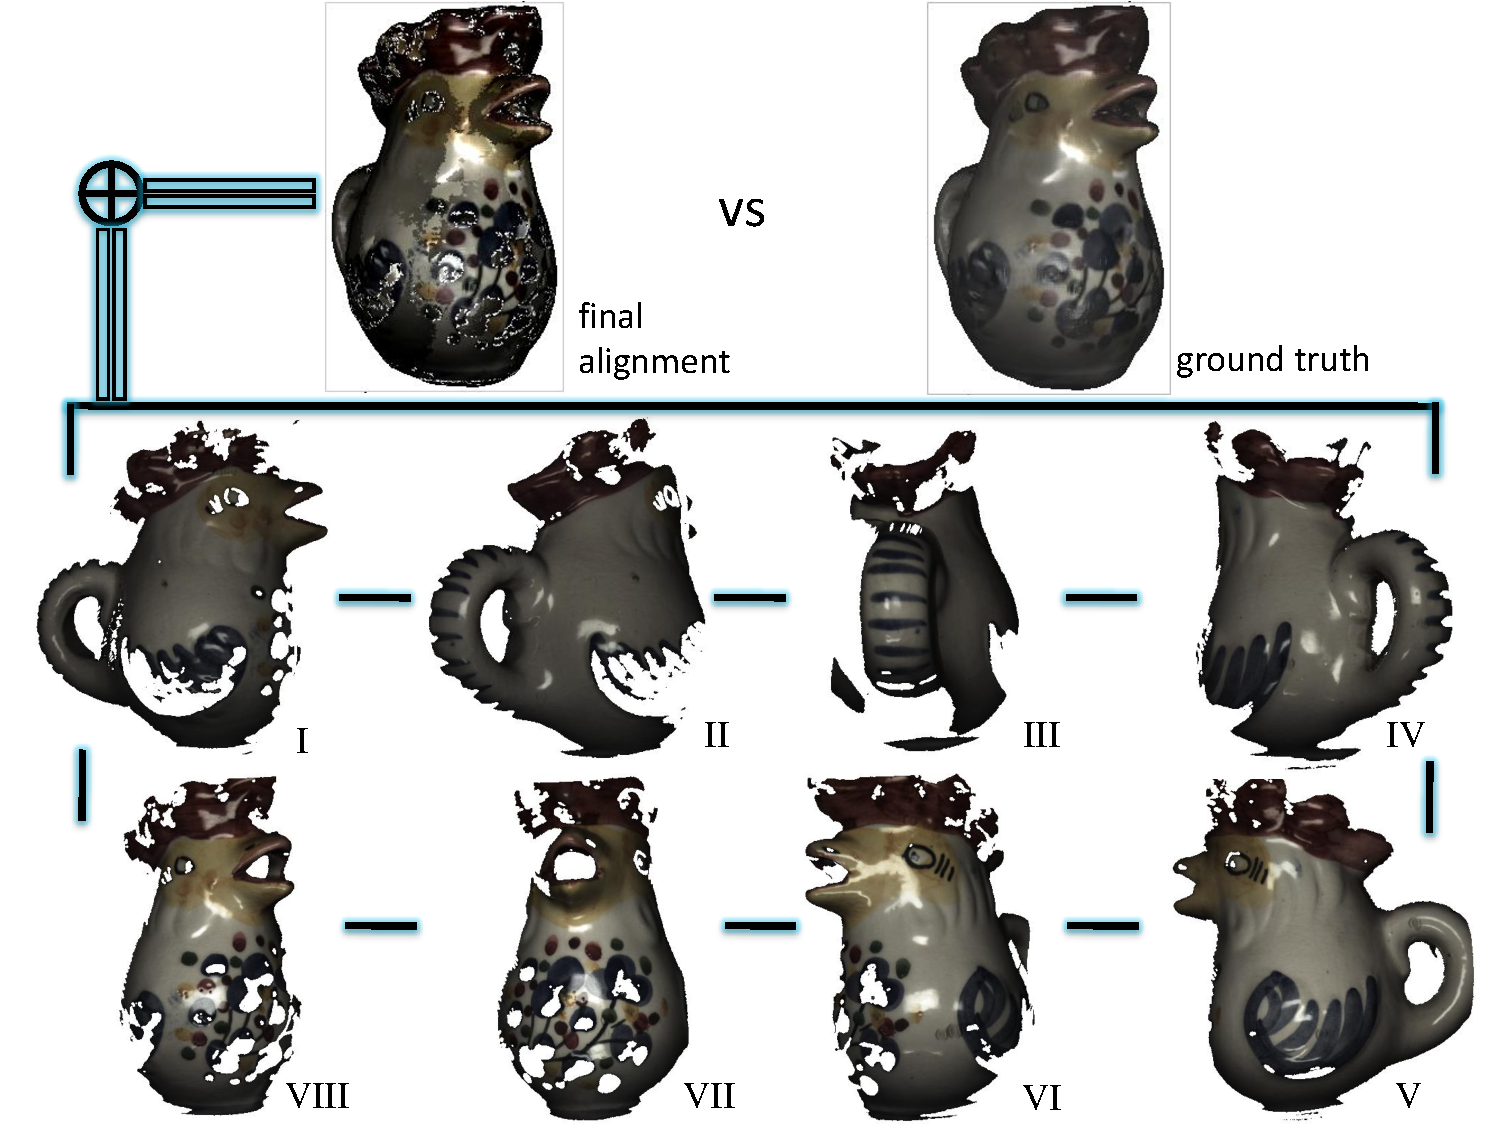
\includegraphics[width=0.99\linewidth]{figures/Rooster.pdf}
  \caption{Alignment of several Rooster scans from different viewpoints.
  Above: our final registered Rooster vs the ground truth [Chuang et al. 2009]. Below: 8 partial scans, the dark lines indicating the pairwise matches.}
\label{fig:3DRigid}
\end{figure}

%%%RRM http://ralph.cs.cf.ac.uk/papers/Geometry/crf.pdf

%-------------------------------------------------------------------------
\subsection{3D Depth Scans with Color Information}
\label{subsec:3dColored}

We next provide a real-world noisy example of the use of SuperMatching.
In this case, real world data with surface color information was captured using a Kinect camera~\cite{Kinect12},
and both SIFT and uniform sampling points were used as a basis for SuperMatching.
This resulted in robust matches without significant outliers, as illustrated in Figure~\ref{fig:3DReal}.
The example also demonstrates that the SuperMatching is general, in the sense that it is independent of feature descriptors.

\begin{figure}[h]
\centering
  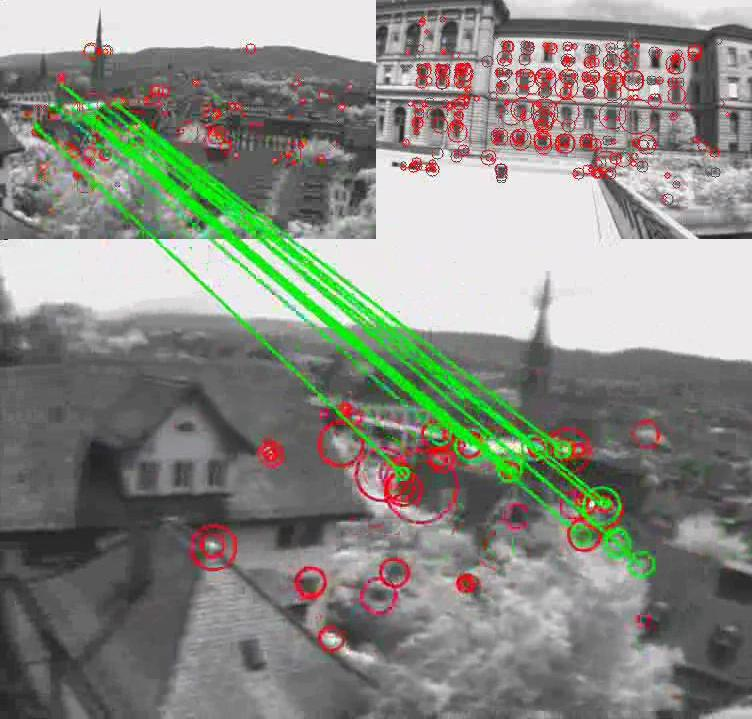
\includegraphics[width=0.9\linewidth]{figures/3DReal.jpg}
  \caption{3D real depth scans with color information, captured using Kinect.
  Above: two given different local pre-scans.  Below: a single scan.
  Matching points are connected by green lines.}
\label{fig:3DReal}
\end{figure}

%-------------------------------------------------------------------------
\subsection{3D Articulated Shape Synthetic Data}
\label{subsec:3darticulated}

Thirdly, we present another application, registration of (approximately) articulated shapes. Such problems are common in dynamic range scanning.
Given a sequence of range scans of a moving articulated subject, our method automatically registers all data to produce a complete 3D shape.
Note that, unlike many other methods, our method does not need  manual segmentation,  markers, or a prior template.
While the problem of non-rigid registration of deformable shapes is ill-posed and no algorithm is applicable to all scenarios,
we believe that our approach pushes the limits of what can be achieved with minimal prior information, and is robust given partial data with holes.

When doing pairwise articulated shape registration,
although the partial scans have missing data and their poses are different, SuperMatching still produces accurate matching.
Correspondences on uniform sampling points on the two shapes are established by SuperMatching;
these permit robust registration of scans by computing piecewise rigid transformations.
These transformations are propagated from the slippage feature points to the entire set of points in each scan using nearest neighbor interpolation.
Figure~\ref{fig:3DRobot} shows two registration examples of an articulated model. 
On the left is our result, on the right is the registered result produced by the method in~\cite{Chang09}.

\begin{figure}[h]
\centering
  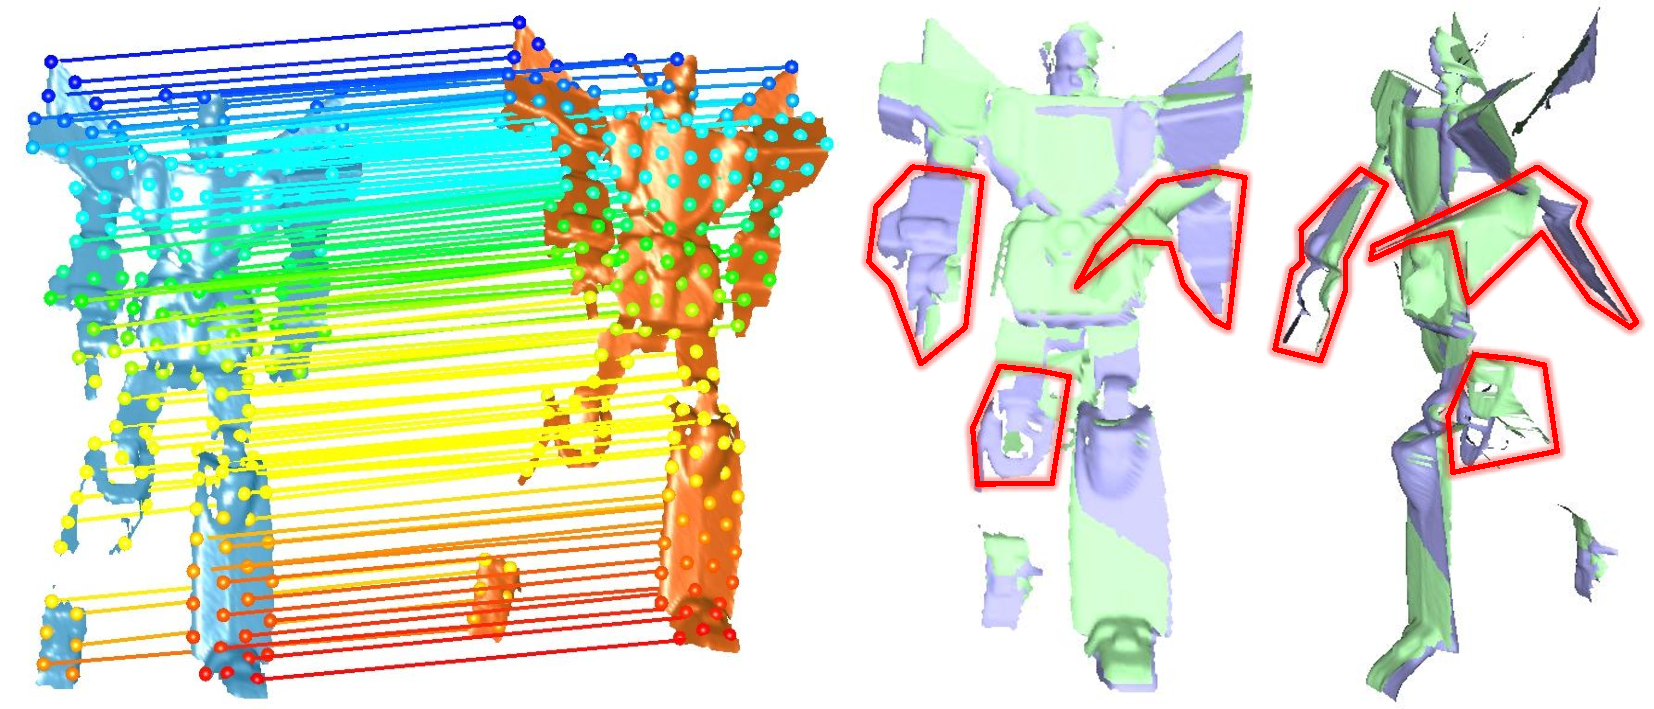
\includegraphics[width=0.95\linewidth]{figures/Robot.pdf}
  \caption{Pairwise matching of articulated Robot between frame 9 and 10. 
           Left: our result. Right: result produced by [Chang and Zwicker 2009] from front and side views, where red polygons indicate the large distortion regions.}
\label{fig:3DRobot}
\end{figure}

For a sequence of partial articulated data, the registration is performed in two main steps.
We first precompute an initial pairwise registration for each pair of consecutive frames, then perform articulated shape reconstruction as in~\cite{Pekelny08}.
Segmentation of the scans into rigid parts can readily be done by clustering the transformations obtained from the slippage feature points,
using the mean shift algorithm~\cite{Comaniciu02}.
This information is used as the input to the second step of articulated shape reconstruction following~\cite{Pekelny08};
this algorithm identifies and tracks the rigid parts in each frame, while accumulating  geometric information over time.
However,~\cite{Pekelny08} requires the user to manually segment each range scan in advance,  whereas we automatically determine  the segmentation.
Figure~\ref{fig:3DHand} shows an articulated hand example.
This synthetic data is generated from a deformation sequence, and the final registered shape is produced from these partial data.
By using synthetic data, we are able to evaluate the robustness of our reconstruction method using the ground truth, as shown in Figure~\ref{fig:3DHand}.
Quantitatively, we measured the maximum of the average distance of the reconstruction over all frames as $0.001 D$ where $D$ is the bounding box diagonal length, and
the greatest distance error in any one frame was $0.012 D$.

\begin{figure}[h]
\centering
  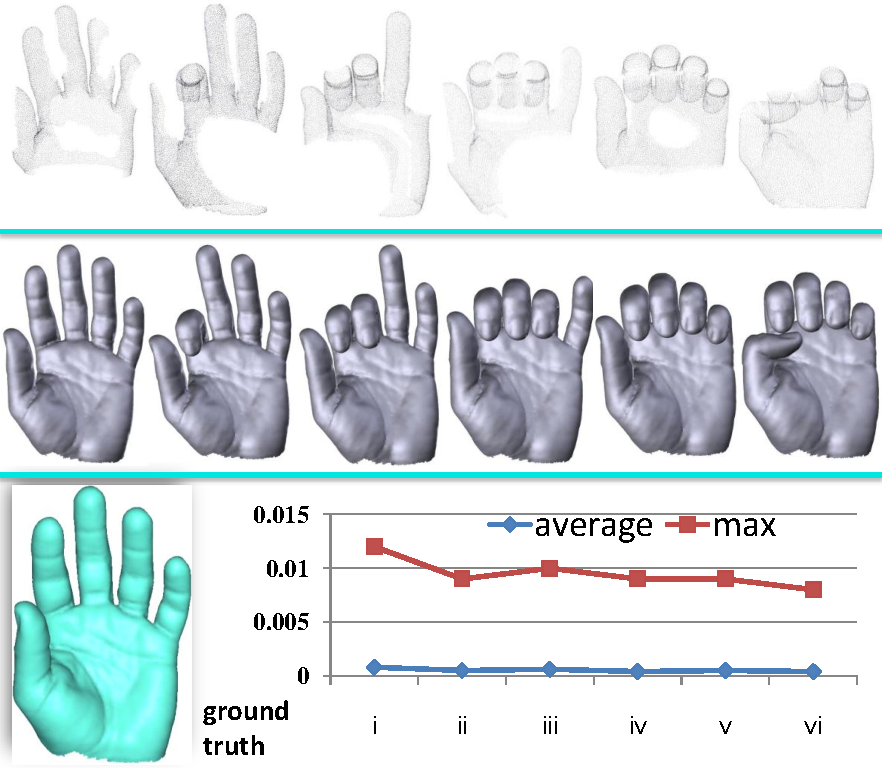
\includegraphics[width=0.95\linewidth]{figures/3DHand.pdf}
  \caption{Registration of an articulated hand.
  Above: partial synthetic data with holes is generated from a deformation sequence.
  The reconstructed meshes are deduced from the registration process (center).
  Below: first frame ground truth shape, and average and maximum distance from the ground truth per frame.}
\label{fig:3DHand}
\end{figure}

%-------------------------------------------------------------------------
\subsection{Deformable Surfaces}
\label{subsec:2DDeformable}

Finally, we matched SIFT points on images of deforming surfaces\footnote{From \url{http://cvlab.epfl.ch/data/dsr/}} showing a cloth and a cushion.
The surface of the cloth underwent relatively smooth deformation, while the surface of the cushion included sharp folds.
This data comes with ground truth, which allows quantitative verification of the accuracy of the matches found.
From each surface set we randomly chose two frames before and after a large deformation.
We randomly chose $100$ corresponding points on each surface, using the provided ground truth.

We used the above input data as a basis for comparison with the spectral algorithm~\cite{Cour06} (a quadratic assignment algorithm),
a third-order tensor algorithm~\cite{Duchenne09},
and the hyper graph matching algorithm~\cite{Zass08}, using the authors' code in each case.
All methods were executed in Matlab on a $2.3$GHz Core2Duo with $2$GB memory.
To enable direct and fair comparison,
~\cite{Duchenne09}, ~\cite{Zass08} and SuperMatching
used the same potential and all used the same tensor size $(N_1N_2)^N$.

In the tests, SuperMatching considered $3\times 10^6$ feature tuples, while the method of~\cite{Duchenne09} considered $10\times 10^6$ features  and the method of~\cite{Zass08} used $4\times 10^6$.
The difference  mainly results from differences in sampling strategy; note that we have the lowest  sampling cost.
The average running time to match two feature sets each with $100$ features was around 8s for SuperMatching, 13s for~\cite{Duchenne09}, 6.5s for~\cite{Zass08}, and 5s for~\cite{Cour06}.
SuperMatching takes less  time than the third-order tensor algorithm in~\cite{Duchenne09} as it uses the same tensor size but fewer feature tuples.

Matching accuracy is assessed by the number of correctly matched points (known from the  ground truth) divided by the total number of points that could be matched.
The results are summarised in Table~\ref{tab:errorrate1} and illustrated in Figure~\ref{fig:2DDeformable}.
Table~\ref{tab:errorrate1} demonstrates that SuperMatching achieves a higher matching accuracy than previous algorithms.
The worst matching result is produced by the spectral quadratic assignment algorithm~\cite{Cour06},
due to the lower discriminatory power of the pairwise geometric constraints used.
Higher-order algorithms perform  better due to the more complex geometric constraints.
Nevertheless, SupeMatching also significantly outperforms the third-order algorithm~\cite{Duchenne09} and the hyper graph matching algorithm~\cite{Zass08}, as these do not tale proper advantage of supersymmetry.

%%%YKL Perhaps compare with [Wang 2010] as well as this test is 2D based.
%%%ZQC Aiping and I did not keep the version submitted to ACCV, during the updating, we directly update the codes by changing the our new equation equ.4.
%%%In fact, aiping is one multiple higher order graph matching, it went beyong previous algorithm by its unified framework without equ. 4 and sampling strategy.

%----------------------------------------
%  deformable matching results IMAGES
%----------------------------------------
%----------------------------------------
\begin{figure}[tb]
\centering
  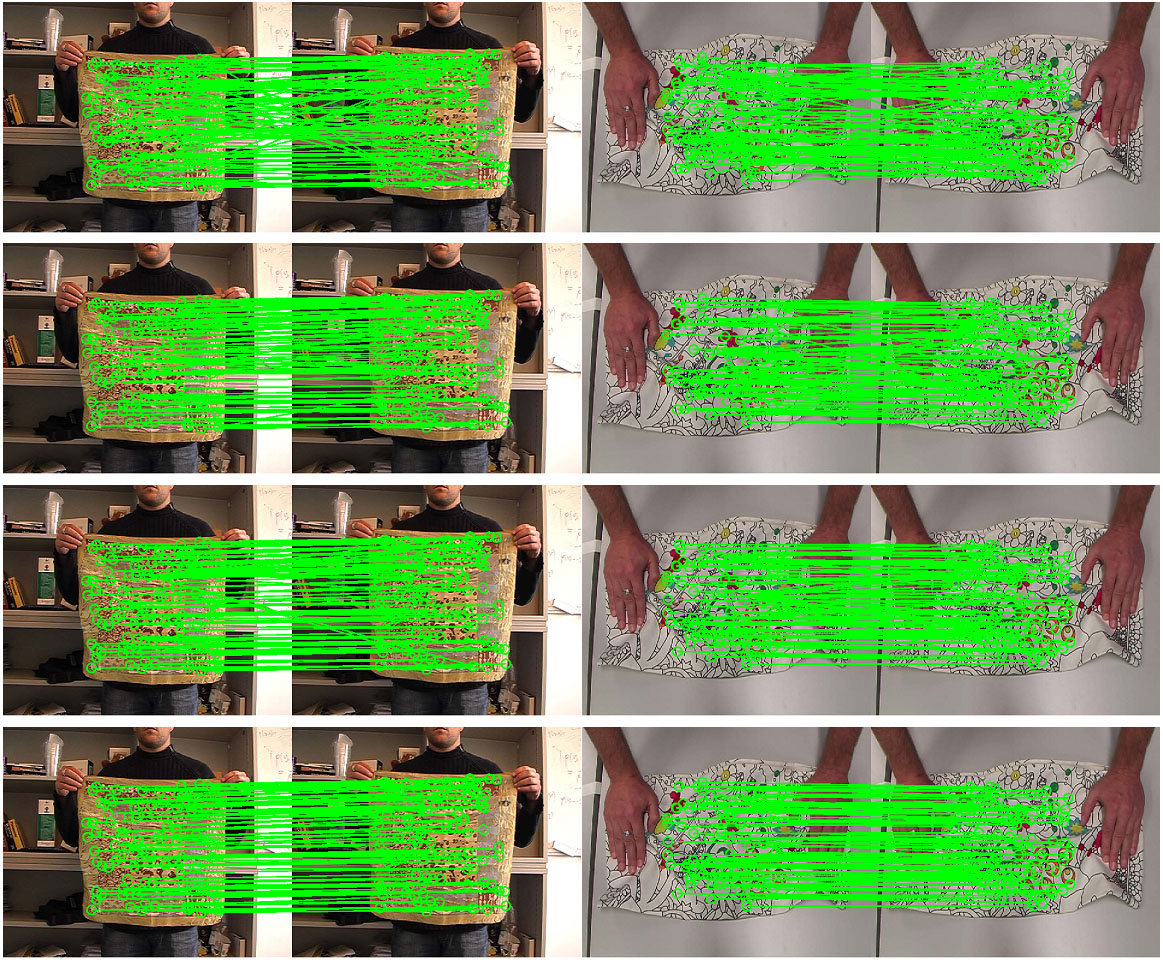
\includegraphics[width=1.00\linewidth]{figures/2DDeformable.jpg}
  \caption{Matching results. Left: cloth set, matching between frame 80 and 90, right: cushion set, matching between 144 and 156.
  Top to bottom, spectral method [Cour et al. 2006], hyper graph matching method [Zass and Shashua 2008], a Third-order tensor [Duchenne et al. 2009], and SuperMatching algorithm.}
\label{fig:2DDeformable}
\end{figure}

%%%RRM This table is too wide. Omit the last two columns
%----------------------------------------
%  deformable matching results TABLE
%----------------------------------------
\begin{table}[tb]
%\vspace{-4mm}
\centering
%\renewcommand{\arraystretch}{0.8}
\tabcolsep=1pt
\setlength{\aboverulesep}{0pt}
\setlength{\belowrulesep}{0pt}
\caption{Accuracy of deformable surface matching.}
\hspace{-5ex}
\label{tab:errorrate1}
\small
\begin{tabular}{l|c c c c | c c c c | c}
\toprule
{Dataset}  & \multicolumn{4}{|c|}{ {cloth}} & \multicolumn{4}{c|}{ {cushion}} & \\
\hline
 {Matching frames} &  {F80-}	&  {F90-}	& {F95-}	& {F100-} & {F144-} & {F156-}	& {F165-}	& {F172-} &  {Time}  \\
 {}                &  {F90 }    &  {F95 }   & {F100}    & {F105}  & {F156}  & {F165}    & {F172}    & {F188}  &  {(s)} \\
\hline
 {SuperMatching}   &  {83\%}    &  {85\%}	& {84\%} 	& {81\%}  & {66\%}	& {60\%}	& {69\%}	& {56\%}  &  {8}  \\
%\hline
 {\cite{Zass08}}   & {73\%}	    & {79\%}	& {70\%}	& {72\%}  & {44\%}  & {39\%}    & {54\%}	& {43\%}   & {6.5}  \\
%\hline
{\cite{Duchenne09}} & {67\%}    & {77\%}    & {73\%}	& {65\%}  & {39\%}	& {31\%}	& {47\%}	& {42\%}   & {13}  \\
%\hline
 {\cite{Cour06}}   & {27\%}     & {29\%}	&  {22\%}	& {27\%}  & {14\%}  & {5\%}	    & {28\%}	& {7\%}    & {5}  \\
\bottomrule
\end{tabular}%
%\vspace{-27pt}
%\vspace{-8mm}
\end{table}%

\section{Conclusion}
\label{sec:conclusion}

This paper has presented the novel SuperMatching algorithm,
which tackles the classic computer graphics and computer vision problem of feature matching, independently of feature description.
It is an efficient higher-order matching algorithm which uses a compact form of the higher-order supersymmetric affinity tensor to express relatedness of features.
Matching is performed using an efficient power iteration method, whose efficiency takes advantage of supersymmetry and avoids computing with zero elements.
We also give an efficient sampling strategy for choosing feature tuples to create the affinity tensor.
Experiments on both synthetic and real 2D and 3D data sets show that
SuperMatching has greater accuracy than competing methods, whilst having competitive performance.

%%===========================================================
%% The Appendices part is started with the command \appendix;
%% appendix sections are then done as normal sections
%\appendix

\textbf{Acknowledgements}. We are grateful to them for sharing related source codes, execution programs, and testing data, whose name would appear after the review.
Then SuperMatching source codes would be public under the GNU Lesser General Public License.
%\section{Why higher-order power iteration solving of supersymmetric tensor is efficient?}
%We explain the idea using a third-order affinity tensor as an example.

% The general matching algorithm finds correspondences considering triangle or higher-order polygons formed by feature points, going beyond traditional pointwise and pairwise approaches. It is formulated as a supersymmetric-tensor-based matching scheme, solved by an efficient higher-order power iteration method. Experiments with several applications demonstrante its accuracy.


%\section*{Acknowledgements}
%
%To Robert, for all the bagels.

\bibliographystyle{acmsiggraph}
\bibliography{fair}
\end{document}
